%\documentstyle[epsf,twocolumn]{jarticle}       %LaTeX2e仕様
\documentclass[twocolumn]{jarticle}     %pLaTeX2e仕様(platex.exeの場合)
%\documentclass[twocolumn]{ujarticle}     %pLaTeX2e仕様(uplatex.exeの場合)
%%%%%%%%%%%%%%%%%%%%%%%%%%%%%%%%%%%%%%%%%%%%%%%%%%%%%%%%%%%%%%
%%
%%  基本バージョン
%%
%%%%%%%%%%%%%%%%%%%%%%%%%%%%%%%%%%%%%%%%%%%%%%%%%%%%%%%%%%%%%%%%
\setlength{\topmargin}{-45pt}
%\setlength{\oddsidemargin}{0cm} 
\setlength{\oddsidemargin}{-7.5mm}
%\setlength{\evensidemargin}{0cm} 
\setlength{\textheight}{24.1cm}
%setlength{\textheight}{25cm} 
\setlength{\textwidth}{17.4cm}
%\setlength{\textwidth}{172mm} 
\setlength{\columnsep}{11mm}

\kanjiskip=.07zw plus.5pt minus.5pt


% 【節が変わるごとに (1.1)(1.2) … (2.1)(2.2) と数式番号をつけるとき】
%\makeatletter
%\renewcommand{\theequation}{%
%\thesection.\arabic{equation}} %\@addtoreset{equation}{section}
%\makeatother

%\renewcommand{\arraystretch}{0.95} 行間の設定

%%%%%%%%%%%%%%%%%%%%%%%%%%%%%%%%%%%%%%%%%%%%%%%%%%%%%%%%
\usepackage[dvipdfmx]{graphicx}   %pLaTeX2e仕様(\documentstyle ->\documentclass)\documentclass[dvipdfmx]{graphicx}
\usepackage[dvipdfmx]{color}
\usepackage[subrefformat=parens]{subcaption}
\usepackage{colortbl}
\usepackage{multicol}
%%%%%%%%%%%%%%%%%%%%%%%%%%%%%%%%%%%%%%%%%%%%%%%%%%%%%%%%

\begin{document}

\twocolumn[
\noindent

\hspace{1em}
\today
\hfill
\ \ 細川 岳大

\vspace{2mm}

\hrule

\begin{center}
{\Large \bf 進捗報告}
\end{center}
\hrule
\vspace{3mm}
]

% ‚ここから 文章 Start!

\section{今週やったこと}

Virtual Adversarial Training(:VAT)の実験をした.
mnistとcifar10について行った.
mnistはラベルあり100枚,ラベルなし49900枚,valdationを10000枚,
modelを中間層のunit数600,1200で活性化関数Reluの三層MLPを用い,
cifar10ではラベルあり4000枚,ラベルなし46000枚,valdationを10000枚,
modelを9層cnnとし,フィルター数96が三層,192が6層で各層でbatchnormalizatoinを,
三層ごとにmaxpoolingとdropoutを入れたmodelとした.

図\ref{fig:graph1},\ref{fig:graph2},
\ref{fig:graph3},\ref{fig:graph4}に結果を示す.

\begin{figure}[h]
	\centering	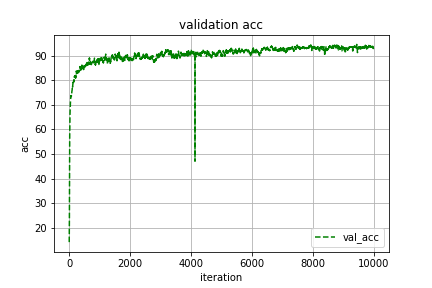
\includegraphics[scale=0.5]{acc__.png}
	\caption{mnistのacc\label{fig:graph1}}
\end{figure}
\begin{figure}[h]
	\centering	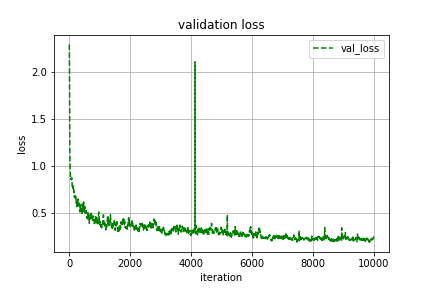
\includegraphics[scale=0.5]{loss__.png}
	\caption{mnistのloss\label{fig:graph2}}
\end{figure}
\begin{figure}[ht]
	\centering	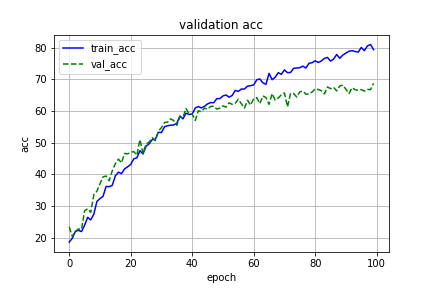
\includegraphics[scale=0.5]{acc_4.png}
	\caption{cifar10のacc\label{fig:graph3}}
\end{figure}
\begin{figure}[ht]
	\centering	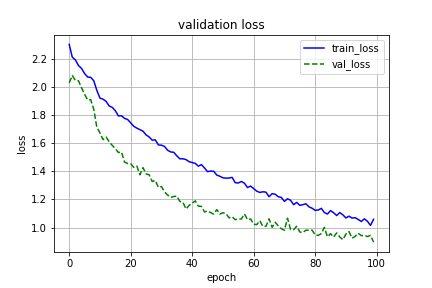
\includegraphics[scale=0.5]{loss_4.png}
	\caption{cifar10のloss\label{fig:graph4}}
\end{figure}

mnistはグラフが少しバグっているが95.2\%までのび,元論文では98.6\%であったのである程度近づけれていた.
一方で,cifar10では70\%程度しか伸びず,論文では85.1\%程度出ており,
若干伸び悩んでいるのが気がかりではある.
\\ \\
また現在FixMatchという手法についても実験中


\section{来週の課題}
\begin{itemize}
	\item 疑似ラベルを加味した実験を行う.
\end{itemize}

\end{document}


